\documentclass{standalone}
\usepackage{tikz}
\usetikzlibrary{patterns, positioning}


\begin{document}
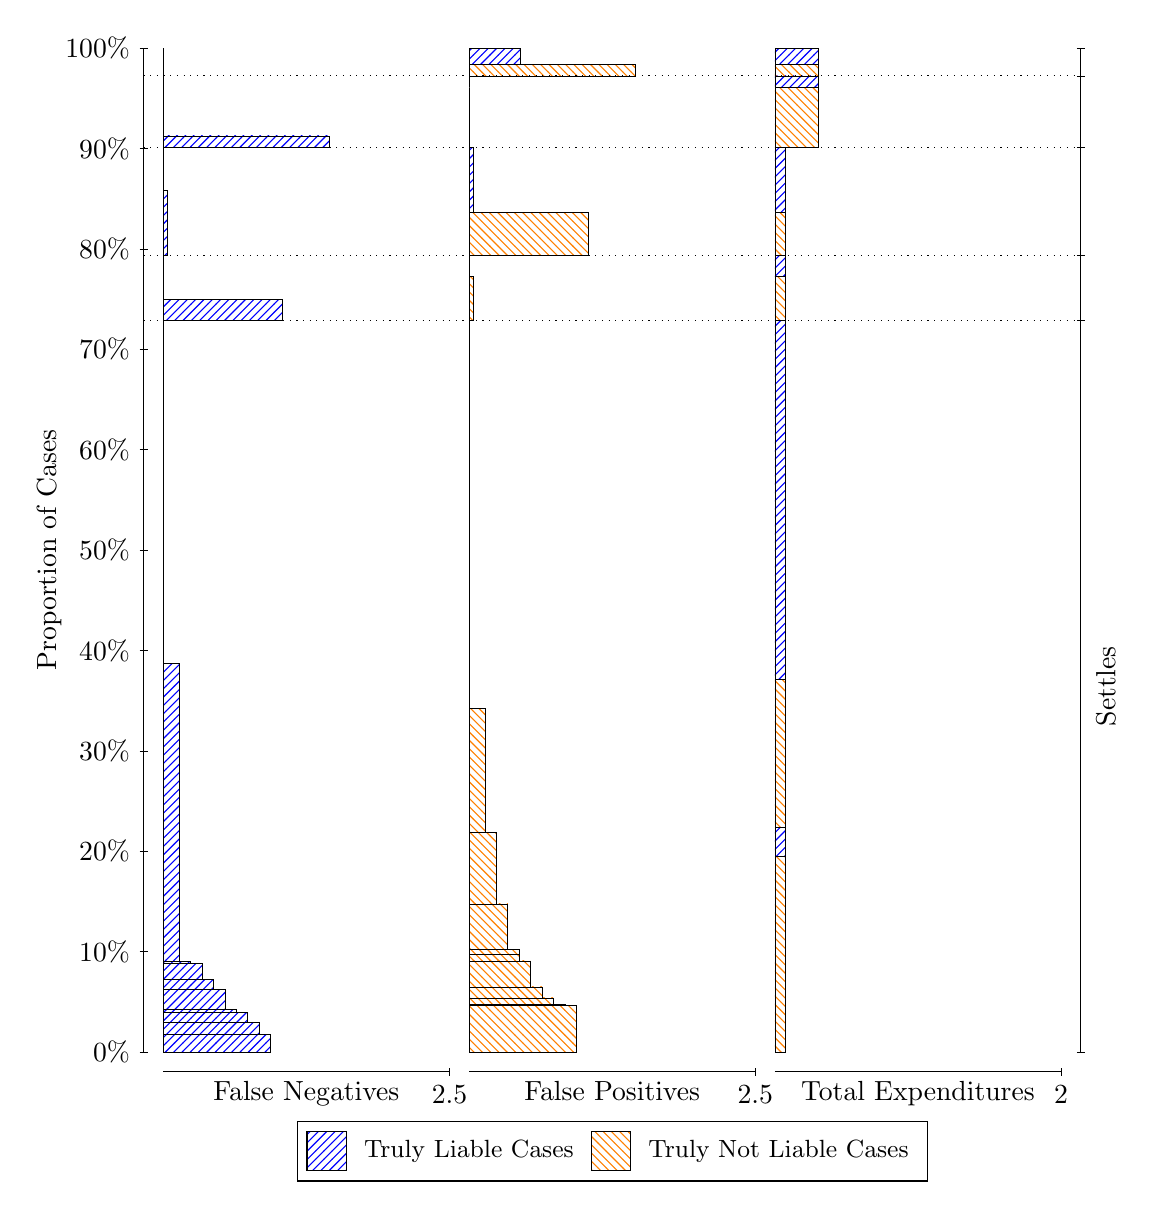
\begin{tikzpicture}
\draw[black, very thin] (1.5,1.75) -- (1.5,14.5);
\node[rotate=90, text=black, anchor=center] at (0.3, 8.125) {Proportion of Cases};
\draw[black, very thin] (1.45,1.75) -- (1.55,1.75);
\node[text=black, anchor=east] at (1.45, 1.75) {0\%};
\draw[black, very thin] (1.45,3.025) -- (1.55,3.025);
\node[text=black, anchor=east] at (1.45, 3.025) {10\%};
\draw[black, very thin] (1.45,4.3) -- (1.55,4.3);
\node[text=black, anchor=east] at (1.45, 4.3) {20\%};
\draw[black, very thin] (1.45,5.575) -- (1.55,5.575);
\node[text=black, anchor=east] at (1.45, 5.575) {30\%};
\draw[black, very thin] (1.45,6.85) -- (1.55,6.85);
\node[text=black, anchor=east] at (1.45, 6.85) {40\%};
\draw[black, very thin] (1.45,8.125) -- (1.55,8.125);
\node[text=black, anchor=east] at (1.45, 8.125) {50\%};
\draw[black, very thin] (1.45,9.4) -- (1.55,9.4);
\node[text=black, anchor=east] at (1.45, 9.4) {60\%};
\draw[black, very thin] (1.45,10.675) -- (1.55,10.675);
\node[text=black, anchor=east] at (1.45, 10.675) {70\%};
\draw[black, very thin] (1.45,11.95) -- (1.55,11.95);
\node[text=black, anchor=east] at (1.45, 11.95) {80\%};
\draw[black, very thin] (1.45,13.225) -- (1.55,13.225);
\node[text=black, anchor=east] at (1.45, 13.225) {90\%};
\draw[black, very thin] (1.45,14.5) -- (1.55,14.5);
\node[text=black, anchor=east] at (1.45, 14.5) {100\%};

\draw[black, very thin] (13.4,1.75) -- (13.4,14.5);
\draw[black, very thin] (13.35,1.75) -- (13.45,1.75);
\node[anchor=west] at (13.35, 1.75) {};
\draw[black, very thin] (13.35,11.041) -- (13.45,11.041);
\node[anchor=west] at (13.35, 11.041) {};
\draw[black, very thin] (13.35,11.868) -- (13.45,11.868);
\node[anchor=west] at (13.35, 11.868) {};
\draw[black, very thin] (13.35,13.235) -- (13.45,13.235);
\node[anchor=west] at (13.35, 13.235) {};
\draw[black, very thin] (13.35,14.147) -- (13.45,14.147);
\node[anchor=west] at (13.35, 14.147) {};
\draw[black, very thin] (13.35,14.5) -- (13.45,14.5);
\node[anchor=west] at (13.35, 14.5) {};

\draw[black, very thin, pattern color=blue, pattern=north east lines] (1.75,1.75) rectangle (3.1125,1.9738);
\draw[black, very thin, pattern color=blue, pattern=north east lines] (1.75,1.9738) rectangle (2.9672,2.1237);
\draw[black, very thin, pattern color=blue, pattern=north east lines] (1.75,2.1237) rectangle (2.8218,2.2508);
\draw[black, very thin, pattern color=blue, pattern=north east lines] (1.75,2.2508) rectangle (2.6765,2.292);
\draw[black, very thin, pattern color=blue, pattern=north east lines] (1.75,2.292) rectangle (2.5312,2.5412);
\draw[black, very thin, pattern color=blue, pattern=north east lines] (1.75,2.5412) rectangle (2.3858,2.6758);
\draw[black, very thin, pattern color=blue, pattern=north east lines] (1.75,2.6758) rectangle (2.2405,2.8727);
\draw[black, very thin, pattern color=blue, pattern=north east lines] (1.75,2.8727) rectangle (2.0952,2.901);
\draw[black, very thin, pattern color=blue, pattern=north east lines] (1.75,2.901) rectangle (1.9498,6.6813);
\draw[black, very thin, pattern color=orange, pattern=north west lines] (1.75,6.6813) rectangle (1.75,11.041);
\draw[black, very thin, pattern color=blue, pattern=north east lines] (1.75,11.041) rectangle (3.2578,11.306);
\draw[black, very thin, pattern color=orange, pattern=north west lines] (1.75,11.306) rectangle (1.75,11.868);
\draw[black, very thin, pattern color=blue, pattern=north east lines] (1.75,11.868) rectangle (1.8045,12.691);
\draw[black, very thin, pattern color=orange, pattern=north west lines] (1.75,12.691) rectangle (1.75,13.235);
\draw[black, very thin, pattern color=blue, pattern=north east lines] (1.75,13.235) rectangle (3.8573,13.385);
\draw[black, very thin, pattern color=orange, pattern=north west lines] (1.75,13.385) rectangle (1.75,14.147);
\draw[black, very thin, pattern color=orange, pattern=north west lines] (1.75,14.147) rectangle (1.75,14.295);
\draw[black, very thin, pattern color=blue, pattern=north east lines] (1.75,14.295) rectangle (1.75,14.5);
\draw[black, very thin, pattern color=orange, pattern=north west lines] (5.6333,1.75) rectangle (6.9958,2.3464);
\draw[black, very thin, pattern color=orange, pattern=north west lines] (5.6333,2.3464) rectangle (6.8505,2.3577);
\draw[black, very thin, pattern color=orange, pattern=north west lines] (5.6333,2.3577) rectangle (6.7052,2.4372);
\draw[black, very thin, pattern color=orange, pattern=north west lines] (5.6333,2.4372) rectangle (6.5598,2.5765);
\draw[black, very thin, pattern color=orange, pattern=north west lines] (5.6333,2.5765) rectangle (6.4145,2.9062);
\draw[black, very thin, pattern color=orange, pattern=north west lines] (5.6333,2.9062) rectangle (6.2692,2.9856);
\draw[black, very thin, pattern color=orange, pattern=north west lines] (5.6333,2.9856) rectangle (6.2692,3.0507);
\draw[black, very thin, pattern color=orange, pattern=north west lines] (5.6333,3.0507) rectangle (6.1238,3.6307);
\draw[black, very thin, pattern color=orange, pattern=north west lines] (5.6333,3.6307) rectangle (5.9785,4.5407);
\draw[black, very thin, pattern color=orange, pattern=north west lines] (5.6333,4.5407) rectangle (5.8332,6.1099);
\draw[black, very thin, pattern color=blue, pattern=north east lines] (5.6333,6.1099) rectangle (5.6333,11.041);
\draw[black, very thin, pattern color=orange, pattern=north west lines] (5.6333,11.041) rectangle (5.6878,11.603);
\draw[black, very thin, pattern color=blue, pattern=north east lines] (5.6333,11.603) rectangle (5.6333,11.868);
\draw[black, very thin, pattern color=orange, pattern=north west lines] (5.6333,11.868) rectangle (7.1412,12.412);
\draw[black, very thin, pattern color=blue, pattern=north east lines] (5.6333,12.412) rectangle (5.6878,13.235);
\draw[black, very thin, pattern color=orange, pattern=north west lines] (5.6333,13.235) rectangle (5.6333,13.997);
\draw[black, very thin, pattern color=blue, pattern=north east lines] (5.6333,13.997) rectangle (5.6333,14.147);
\draw[black, very thin, pattern color=orange, pattern=north west lines] (5.6333,14.147) rectangle (7.7407,14.295);
\draw[black, very thin, pattern color=blue, pattern=north east lines] (5.6333,14.295) rectangle (6.2873,14.5);
\draw[black, very thin, pattern color=orange, pattern=north west lines] (9.5167,1.75) rectangle (9.6529,4.2292);
\draw[black, very thin, pattern color=blue, pattern=north east lines] (9.5167,4.2292) rectangle (9.6529,4.6029);
\draw[black, very thin, pattern color=orange, pattern=north west lines] (9.5167,4.6029) rectangle (9.6529,6.4837);
\draw[black, very thin, pattern color=blue, pattern=north east lines] (9.5167,6.4837) rectangle (9.6529,11.041);
\draw[black, very thin, pattern color=orange, pattern=north west lines] (9.5167,11.041) rectangle (9.6529,11.603);
\draw[black, very thin, pattern color=blue, pattern=north east lines] (9.5167,11.603) rectangle (9.6529,11.868);
\draw[black, very thin, pattern color=orange, pattern=north west lines] (9.5167,11.868) rectangle (9.6529,12.412);
\draw[black, very thin, pattern color=blue, pattern=north east lines] (9.5167,12.412) rectangle (9.6529,13.235);
\draw[black, very thin, pattern color=orange, pattern=north west lines] (9.5167,13.235) rectangle (10.062,13.997);
\draw[black, very thin, pattern color=blue, pattern=north east lines] (9.5167,13.997) rectangle (10.062,14.147);
\draw[black, very thin, pattern color=orange, pattern=north west lines] (9.5167,14.147) rectangle (10.062,14.295);
\draw[black, very thin, pattern color=blue, pattern=north east lines] (9.5167,14.295) rectangle (10.062,14.5);
\draw[black, dotted] (1.5,11.041) -- (13.4,11.041);
\draw[black, dotted] (1.5,11.868) -- (13.4,11.868);
\draw[black, dotted] (1.5,13.235) -- (13.4,13.235);
\draw[black, dotted] (1.5,14.147) -- (13.4,14.147);
\draw[black, very thin] (1.75,1.5) -- (5.3833,1.5);
\node[text=black, anchor=north] at (3.5667, 1.5) {False Negatives};
\draw[black, very thin] (5.3833,1.45) -- (5.3833,1.55);
\node[text=black, anchor=north] at (5.3833, 1.45) {2.5};

\draw[black, very thin] (5.6333,1.5) -- (9.2667,1.5);
\node[text=black, anchor=north] at (7.45, 1.5) {False Positives};
\draw[black, very thin] (9.2667,1.45) -- (9.2667,1.55);
\node[text=black, anchor=north] at (9.2667, 1.45) {2.5};

\draw[black, very thin] (9.5167,1.5) -- (13.15,1.5);
\node[text=black, anchor=north] at (11.333, 1.5) {Total Expenditures};
\draw[black, very thin] (13.15,1.45) -- (13.15,1.55);
\node[text=black, anchor=north] at (13.15, 1.45) {2};

\node[text=black, centered, rotate=90] at (13.72, 6.3956) {Settles};





\draw (7.449999999999999,1.5) node[draw=none] (baseCoordinate) {};
\begin{scope}[align=center]
        \matrix[scale=0.5, draw=black, below=0.5cm of baseCoordinate, nodes={draw}, column sep=0.1cm]{
            \node[rectangle, draw, minimum width=0.5cm, minimum height=0.5cm, pattern color=blue, pattern=north east lines] {}; &
            \node[draw=none, font=\small, text=black] (B) {Truly Liable Cases}; &
            \node[rectangle, draw, minimum width=0.5cm, minimum height=0.5cm, pattern color=orange, pattern=north west lines] {}; &
            \node[draw=none, font=\small, text=black] (B) {Truly Not Liable Cases}; \\
            };
\end{scope}

\end{tikzpicture}
\end{document}